%Config
\documentclass[12pt,twoside]{article}
\usepackage[spanish,es-tabla]{babel}
\usepackage[a4paper]{geometry}

\usepackage{graphicx}               % Para incluir imágenes
\usepackage{amsmath}                % Para el manejo de matemáticas
\usepackage{url}
\usepackage{enumitem}
\usepackage{float}

\title{La hormiga de Langton y la interacción entre diferentes hormigueros}
\author{Erick Jesse Angeles López}


% Definir un comando para palabras clave
\newcommand{\keywords}[1]{%
	\begin{center}
		\textbf{Palabras clave:} #1
	\end{center}
}

\renewcommand{\baselinestretch}{1}
\setcounter{page}{1}
\setlength{\textheight}{21.6cm}
\setlength{\textwidth}{14cm}
\setlength{\oddsidemargin}{1cm}
\setlength{\evensidemargin}{1cm}
\pagestyle{myheadings}
\thispagestyle{empty}
\markboth{\small{Ángeles López Erick Jesse}}{\small{La hormiga de Langton y la interacción entre diferentes hormigueros}}
\date{}

\begin{document}
	
	\begin{center}
		
		% Contenido izquierdo - Imagen
		\begin{minipage}{0.17\textwidth}
			\centering
			
\includegraphics[width=0.7\textwidth]{img/ipn_logo.jpg} % Ajusta esta línea
		\end{minipage}
		\begin{minipage}{.55\textwidth}
			\centering
			{\Large Instituto Politécnico Nacional}\\
			{\Large Escuela Superior de Cómputo}
		\end{minipage}
		\begin{minipage}{0.17\textwidth}
			\centering
			
\includegraphics[width=0.9\textwidth]{img/escom_logo} % Ajusta esta línea
		\end{minipage}			
	\end{center}
	
	
	\centerline{\bf Ingeniería en Inteligencia Artificial, Algoritmos bioinspirados}
	
	\centerline{\bf  Sem: 2025-1, 5BM1, Fecha: 6-Enero-2025}
	
	\centerline{}
	
	%\centerline{}
	
	
	\begin{center}
		\Large{\textsc{La Hormiga de Langton y la interacción entre diferentes hormigueros}} 
	\end{center}
	\centerline{}
	\centerline{\bf {\textit{Presenta}}}
	\centerline{\bf {Angeles López Erick Jesse\footnote{eangelesl1700@alumno.ipn.mx}}}
	\centerline{}
	\centerline{}
	\centerline{\bf {Disponible en:}}
	\centerline{\text{\url{GITHUB}}}
	
	
	
	
	\newtheorem{Theorem}{\quad Theorem}[section]
	
	\newtheorem{Definition}[Theorem]{\quad Definition}
	
	\newtheorem{Corollary}[Theorem]{\quad Corollary}
	
	\newtheorem{Lemma}[Theorem]{\quad Lemma}
	
	\newtheorem{Example}[Theorem]{\quad Example}
	
	\bigskip
	
	\bigskip
	
	\begin{abstract} 
		
	\end{abstract}
	
	\keywords{}
	
	\clearpage
	
	\tableofcontents
	\clearpage
	
	\clearpage
	\section{Introducción}
	
	La hormiga de Langton, creada por Chris Langton en 1986, es un modelo computacional sencillo que genera comportamientos emergentes y patrones complejos a partir de reglas simples. Originalmente, la hormiga sigue dos reglas básicas que dan lugar a un comportamiento caótico e impredecible. Este modelo es un excelente ejemplo de sistemas dinámicos en los que reglas locales producen estructuras globales.
	
	En esta práctica, exploramos el comportamiento de la hormiga de Langton bajo diferentes condiciones, como cambios en las reglas, la interacción de múltiples hormigas en un mismo espacio y el establecimiento de colonias. Nuestro objetivo es analizar las dinámicas emergentes y las densidades de los estados en el tablero, así como estudiar la expansión del área inicial ocupada por las hormigas. Para ello, se diseñó un software específico que permite realizar simulaciones personalizadas y graficar los resultados.
	
	\section{Marco Teórico}
	
	\subsection{Funcionamiento de la Hormiga de Langton}
	
	La hormiga de Langton se desplaza sobre una cuadrícula bidimensional (teóricamente infinita) en la que cada celda puede tener un estado de 0 o 1. Sigue dos reglas simples:  
	\begin{enumerate}
		\item Si la hormiga está en una celda con estado 0:
		\begin{itemize}
			\item Cambia el estado de la celda a 1.
			\item Gira 90° a la derecha y avanza.
		\end{itemize}
		\item Si la hormiga está en una celda con estado 1:
		\begin{itemize}
			\item Cambia el estado de la celda a 0.
			\item Gira 90° a la izquierda y avanza.
		\end{itemize}
	\end{enumerate}
	
	Esta configuración inicial se conoce como la regla \textbf{RL}, donde:  
	\begin{itemize}
		\item El tamaño de la regla define el número de estados consecutivos, en este caso $\{0, 1\}$.  
		\item \textbf{R} y \textbf{L} indican giros a la derecha (\textbf{Right}) e izquierda (\textbf{Left}), respectivamente.  
		\item El nuevo estado es el consecutivo en el ciclo. Por ejemplo, del estado 0 pasa al estado 1, y del estado 1 regresa al estado 0.  
	\end{itemize}
	
	Bajo esta estructura, pueden definirse múltiples reglas, como la regla \textbf{LLR}, que sigue estas instrucciones:  
	\begin{itemize}[noitemsep]
		\item Si el estado es 0, gira a la izquierda.  
		\item Si el estado es 1, gira a la izquierda.  
		\item Si el estado es 2, gira a la derecha.  
	\end{itemize}
	
	\subsection{Clasificación: Agente y Autómata Celular}
	
	La hormiga de Langton puede ser catalogada tanto como un agente como un autómata celular:  
	\begin{itemize}
		\item \textbf{Agente}: Es una entidad autónoma que toma decisiones individuales basadas en ciertas reglas, lo que coincide con el comportamiento definido anteriormente de la hormiga.  
		\item \textbf{Autómata celular}: Un sistema dinámico compuesto por celdas que cambian de estado según una vecindad y una función de transición. Aunque la definición no parece encajar perfectamente, el comportamiento de la hormiga puede replicarse definiendo estados y reglas específicas.  
	\end{itemize}
	
	Por ejemplo, para la regla \textbf{RL}, el autómata celular equivalente se define de la siguiente manera: 
	\begin{itemize}
		\item \textbf{Dimensión}: Plano bidimensional.  
		\item \textbf{Estados}: Se extienden los estados originales $\{0, 1\}$ para incluir información sobre la dirección de la hormiga: $\{0, 0_U, 0_D, 0_L, 0_R, 1, 1_U, 1_D, 1_L, 1_R\}$, donde el subíndice indica la dirección.  
		\item \textbf{Vecindad}: Vecindad de Neumann (los cuatro vecinos ortogonales más cercanos y la celda central).  
		\item \textbf{Función de transición}: Las reglas incluyen:  
		\begin{itemize}
			\item Si una celda contiene una hormiga, su estado cambia al estado sin hormiga:  
			\[ c(t) = x_y \rightarrow c(t+1) = x \]  
			\item Si una celda vecina contiene una hormiga mirando hacia ella, adquiere el estado correspondiente con la nueva dirección. Por ejemplo, a continuación se define el comportamiento de una celda si su vecina izquierda tiene una hormiga mirando a la derecha:  
			\[
			c_{(-1, 0)}(t) = x_R, c(t) = 0 \rightarrow c(t+1) = 1_D, \: \forall x \in \text{Estados iniciales}
			\]
			\[
			c_{(-1, 0)}(t) = x_R, c(t) = 1 \rightarrow c(t+1) = 0_U, \: \forall x \in \text{Estados iniciales}
			\]
		\end{itemize}
	\end{itemize}
	
	Este autómata celular esta diseñado unicamente para una hormiga.
	
\section{Objetivo de la Práctica}

El objetivo de esta práctica es estudiar los siguientes aspectos:  
\begin{itemize}
	\item El impacto de diferentes reglas sobre el comportamiento de las hormigas.  
	\item Las interacciones entre múltiples hormigas en un mismo espacio.  
	\item La formación, el comportamiento y la interacción entre colonias independientes.  
\end{itemize}

Durante las pruebas, se analizarán y graficarán las densidades de los estados de las celdas y la expansión desde el punto inicial. Las simulaciones se llevaron a cabo utilizando un software desarrollado específicamente para esta práctica, detallado en la sección de metodología.

\clearpage
\section{Metodología}

\subsection{Diseño de Software}

El software fue desarrollado en C++ utilizando el proyecto \textit{Graphic Mode}, que implementa interfaces gráficas mediante la librería SFML. Este programa incorpora múltiples elementos esenciales para la práctica, tales como:  
\begin{itemize}
	\item Creación y manipulación de \textit{frames}.
	\item Implementación de botones interactivos.
	\item Campos de texto para la entrada de datos.
	\item Representación de cuadrículas y gráficas.
\end{itemize}

Estas herramientas permiten diseñar un entorno visual adecuado para simular, visualizar y analizar el comportamiento de las hormigas de Langton.

\subsection{Comportamiento de una sola Hormiga de Langton}

La hormiga de Langton, en su versión tradicional, opera bajo la regla \textbf{RL}, definida de la siguiente manera:  
\begin{itemize}
	\item Si el estado de la casilla es 0, la hormiga gira a la derecha.  
	\item Si el estado de la casilla es 1, la hormiga gira a la izquierda.  
\end{itemize}

Este sencillo conjunto de reglas produce dos dinámicas características:  
\begin{enumerate}
	\item Un comportamiento inicial caótico y aparentemente aleatorio.  
	\item La formación de un patrón cíclico denominado ``carretera", que permite a la hormiga expandirse de forma infinita en una dirección.  
\end{enumerate}

En la Figura \ref{img:rl1} se muestra el resultado del movimiento de una hormiga tras completar 10,000 pasos. Posteriormente, en la Figura \ref{img:rl2}, se observa cómo la carretera se desarrolla casi de manera inmediata, permitiendo un crecimiento constante desde ese punto. 

Cada gráfico utiliza colores para representar los diferentes estados, con las casillas negras indicando áreas no visitadas, que no poseen un estado asignado.

\begin{figure}[H]
	\centering
	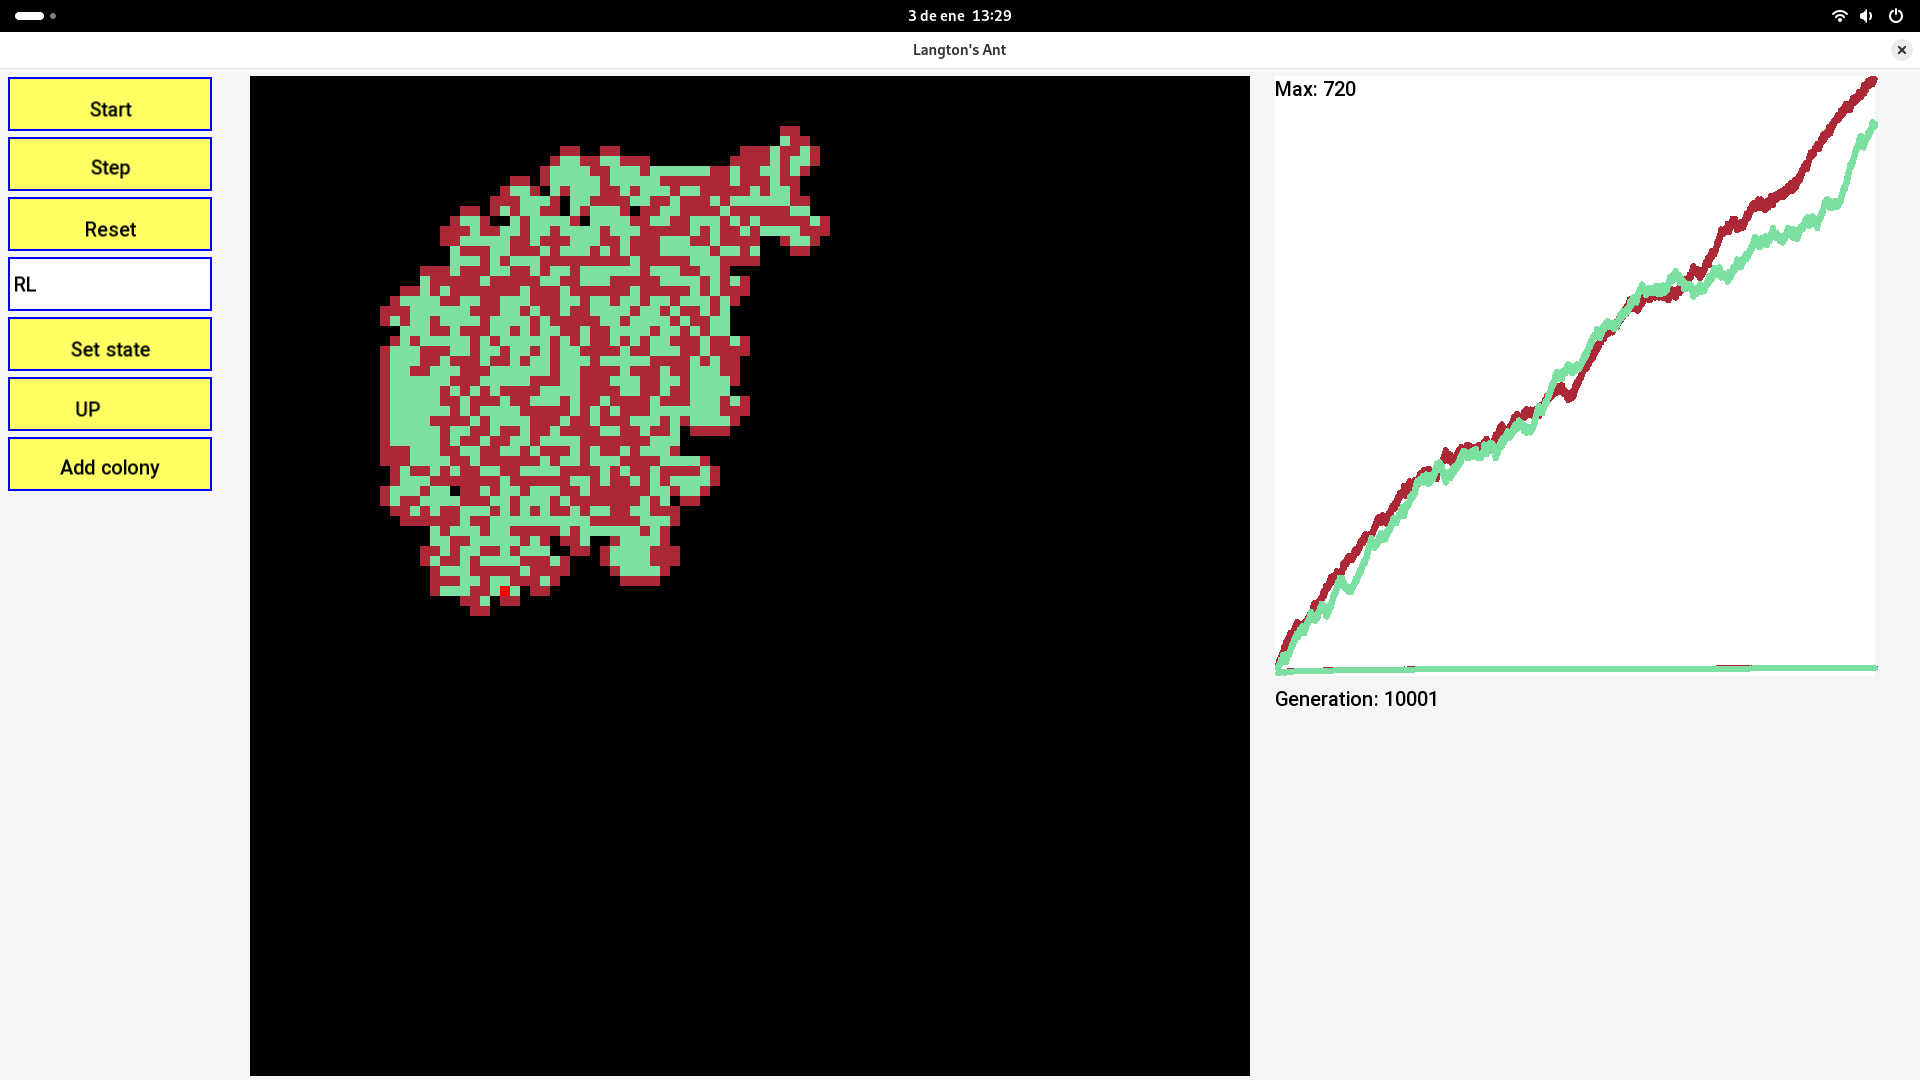
\includegraphics[width=\textwidth]{img/rl1.png}
	\caption{Movimiento inicial de una hormiga bajo la regla RL (10,000 pasos).}
	\label{img:rl1}
\end{figure}

\begin{figure}[H]
	\centering
	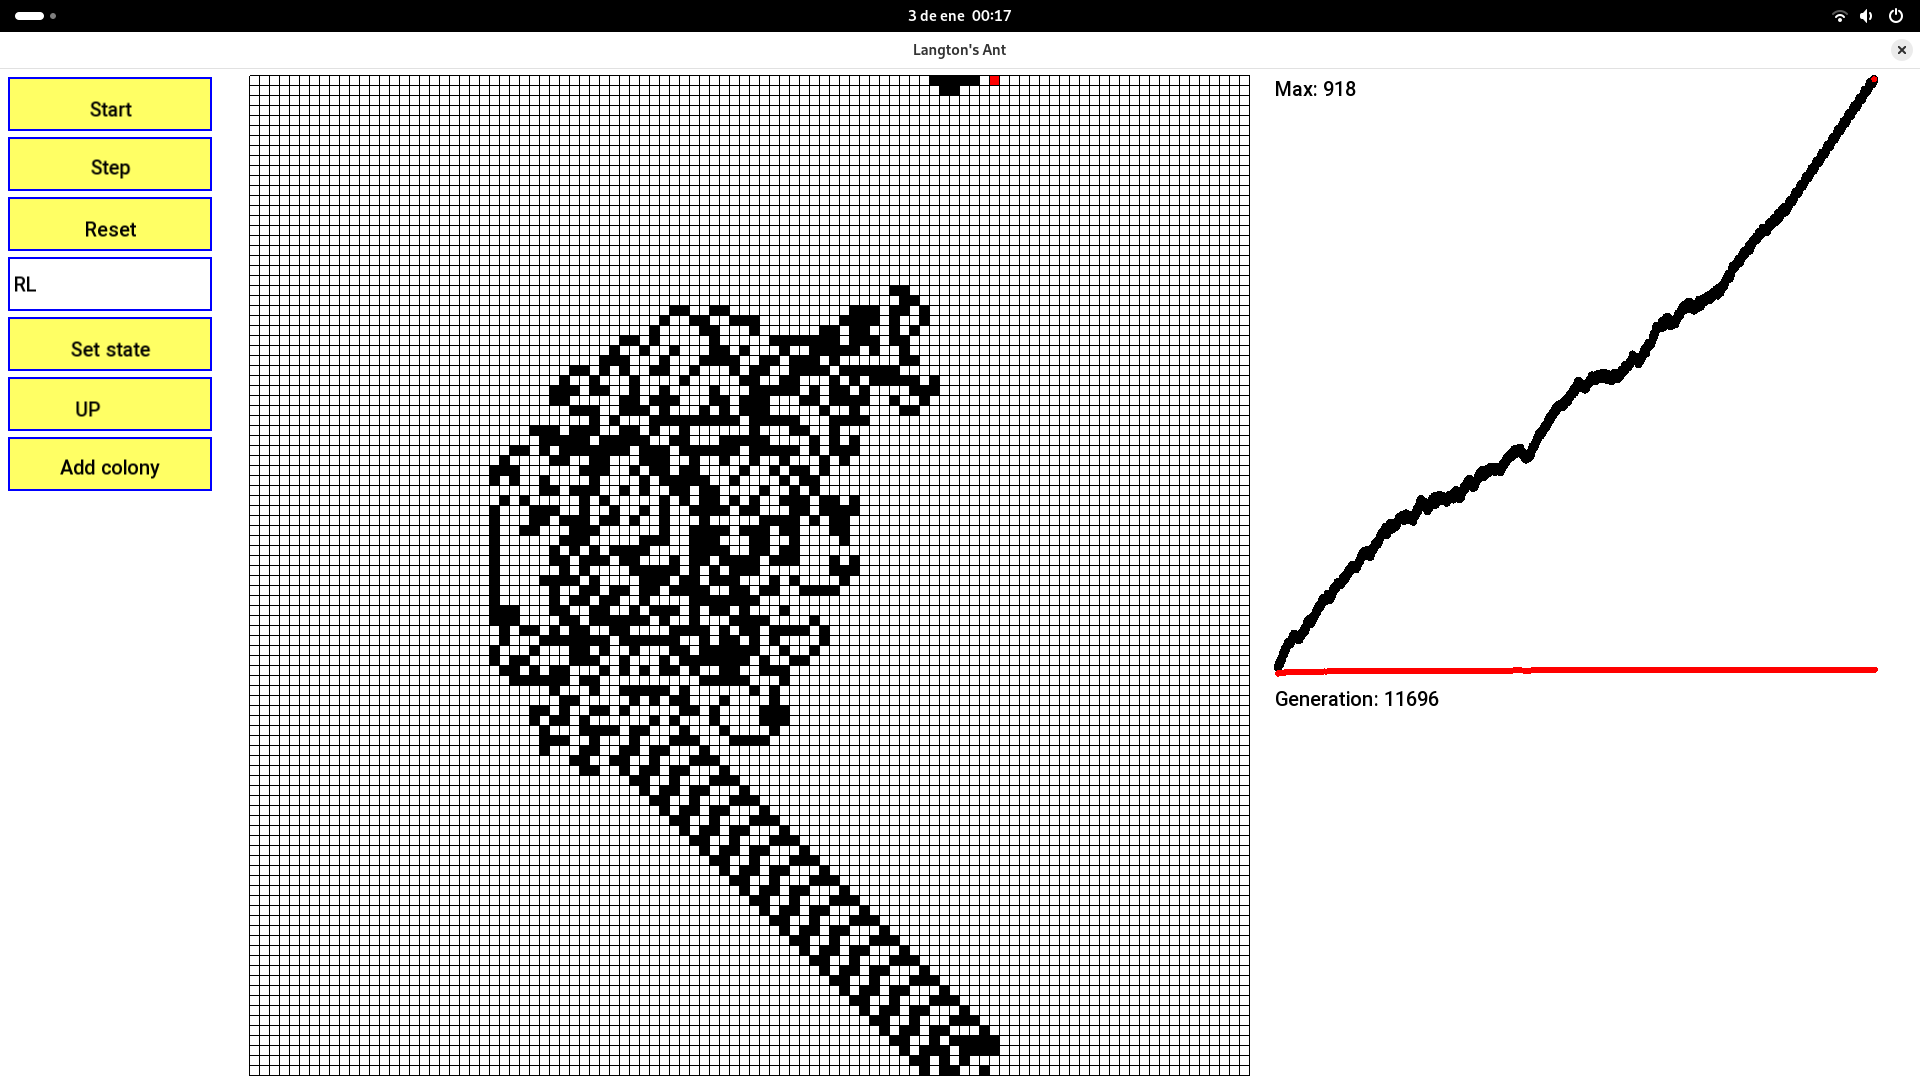
\includegraphics[width=\textwidth]{img/rl2.png}
	\caption{Construcción de la carretera por una hormiga bajo la regla RL.}
	\label{img:rl2}
\end{figure}

Como se mencionó previamente, las hormigas de Langton pueden operar con diversas reglas, lo que permite modelar y analizar comportamientos variados en un espacio bidimensional. A continuación, en la Figura \ref{fig:rules}, se presentan configuraciones generadas con distintas reglas. Algunas de estas reglas permiten la creación de carreteras de manera casi inmediata.

\begin{figure}[h!]
	\centering
	% Primera fila: Regla LLR
	\begin{minipage}{0.45\textwidth}
		\centering
		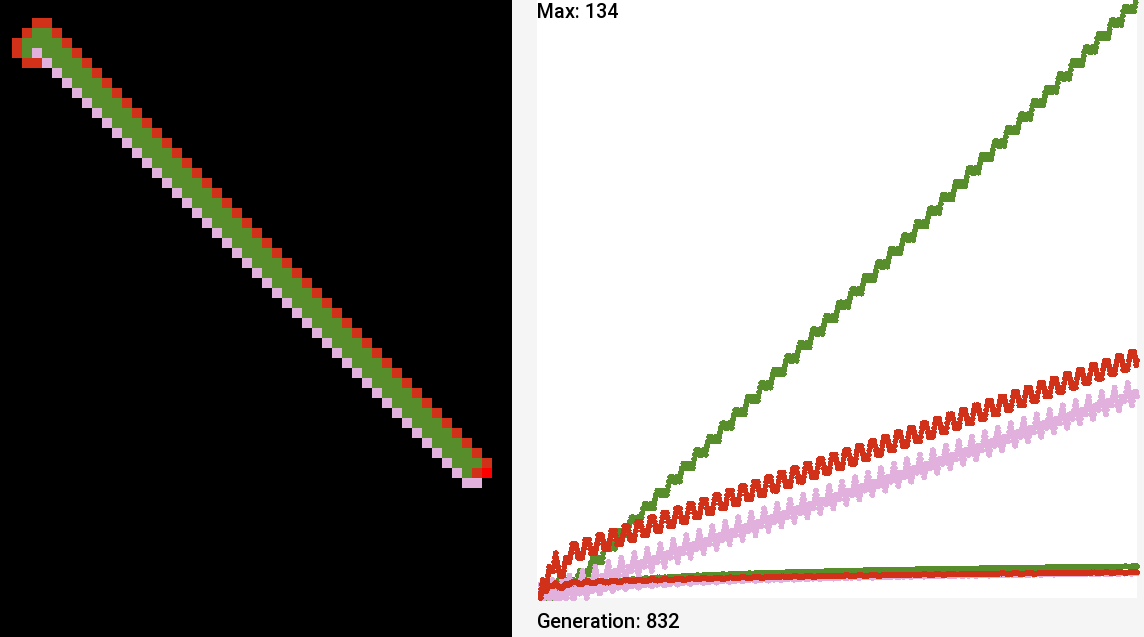
\includegraphics[width=\textwidth]{img/llr1.png}
	\end{minipage}%
	\hspace{0.5cm}%
	\begin{minipage}{0.45\textwidth}
		\centering
		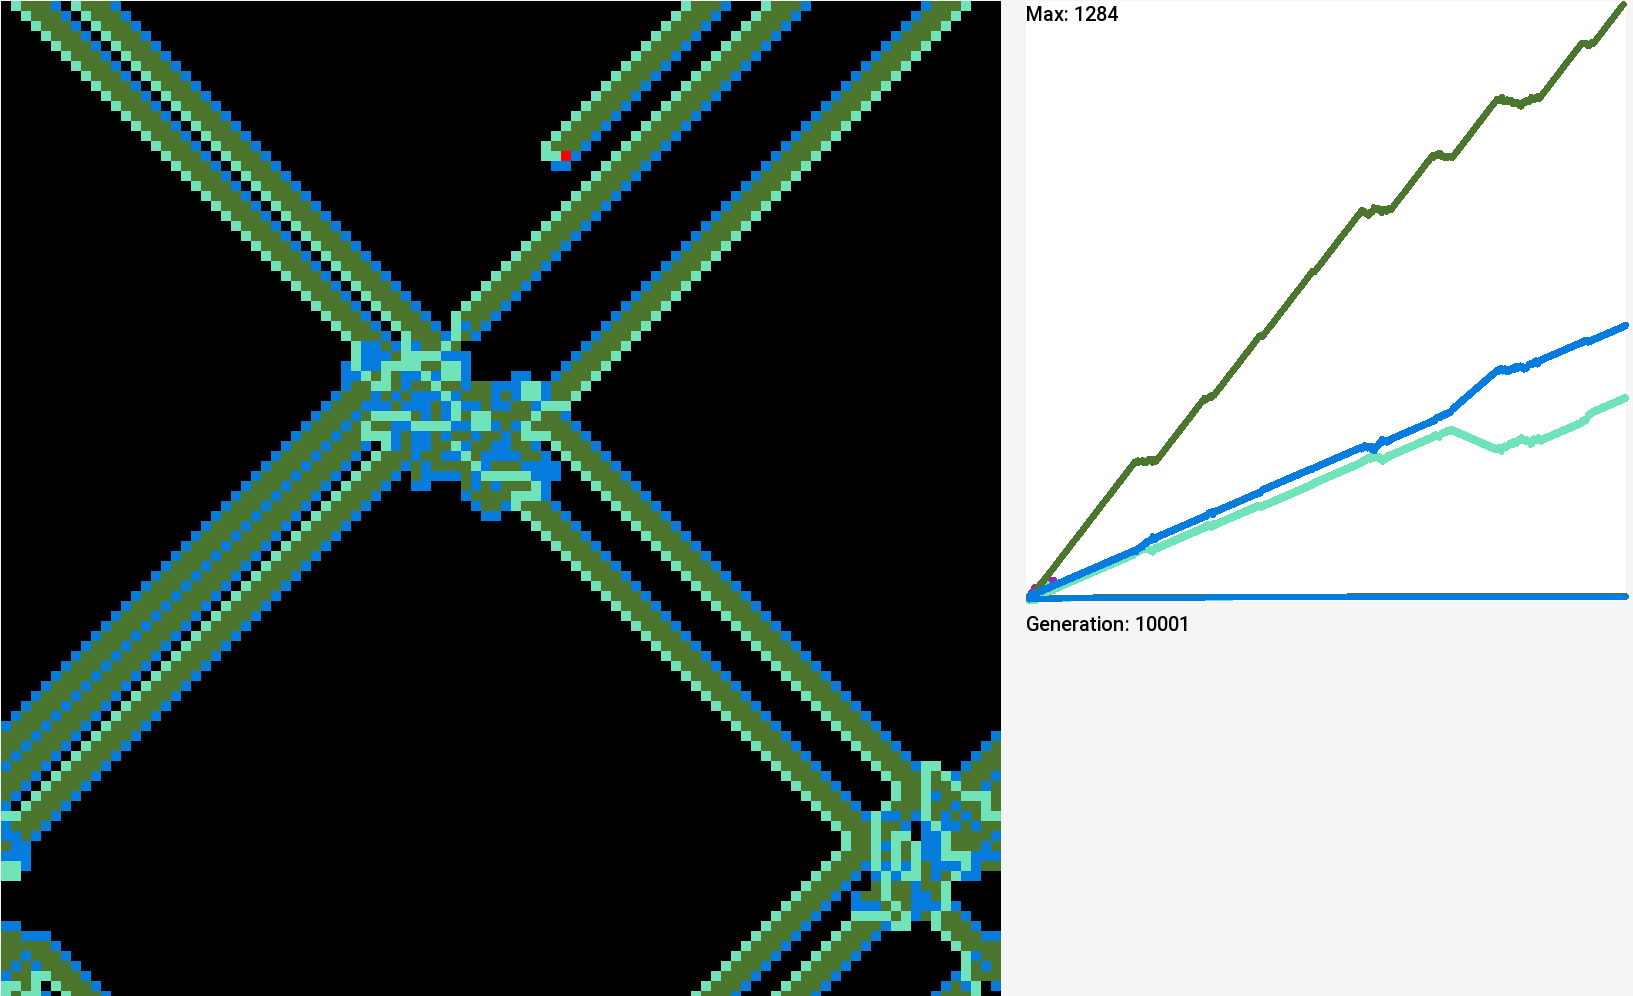
\includegraphics[width=\textwidth]{img/llr2.png}
	\end{minipage}
	\vspace{0.3cm}
	
	\begin{minipage}{0.9\textwidth}
		\centering
		\small La regla LLR crea carreteras de forma casi inmediata. Incluso tiene la capacidad de añadir carriles en carreteras existentes. Las perturbaciones en la gráfica representan colisiones con otros elementos en el espacio, aunque, generalmente, se necesitan pocas generaciones para que la hormiga recupere su trayectoria.
	\end{minipage}
	\vspace{0.5cm}
	
	% Segunda fila: Regla RLLR
	\begin{minipage}{0.45\textwidth}
		\centering
		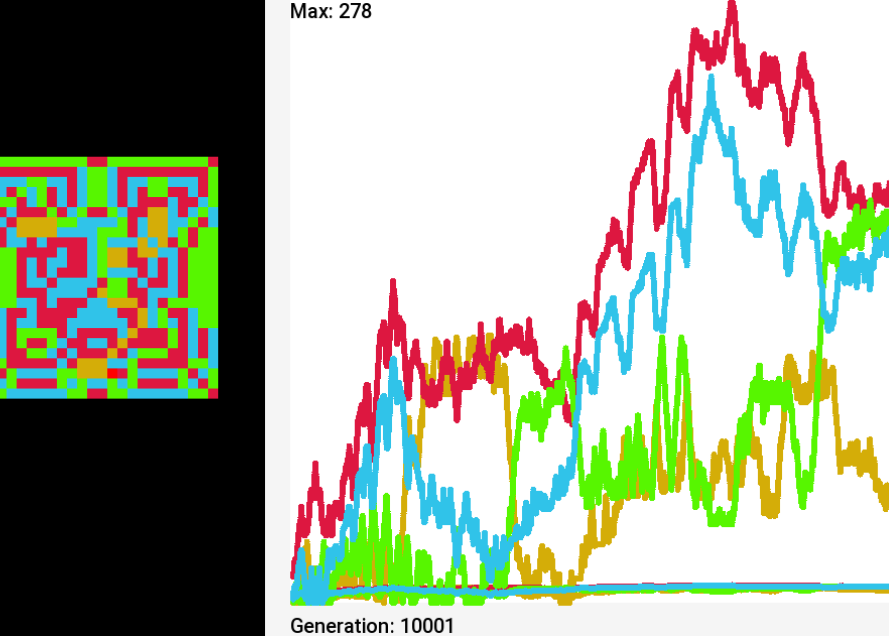
\includegraphics[width=\textwidth]{img/rllr1.png}
	\end{minipage}%
	\hspace{0.5cm}%
	\begin{minipage}{0.45\textwidth}
		\centering
		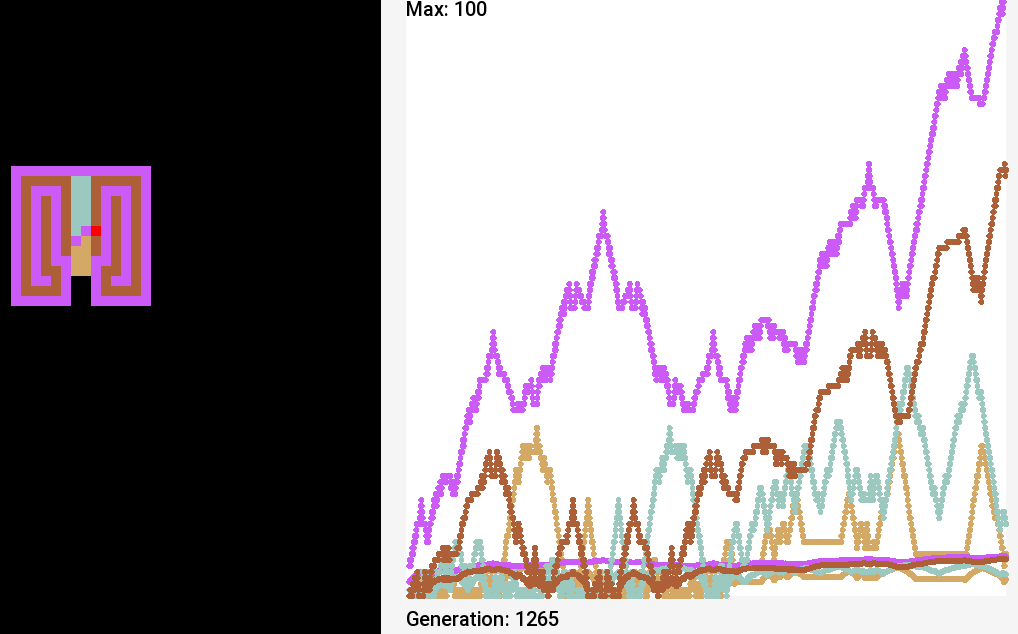
\includegraphics[width=\textwidth]{img/rllr2.png}
	\end{minipage}
	\vspace{0.3cm}
	
	\begin{minipage}{0.9\textwidth}
		\centering
		\small La regla RLLR se desarrolla en forma cuadrada y no crece hasta que la estructura interna ha cambiado casi por completo. Además, a diferencia de las reglas anteriores, las densidades de estado en esta regla presentan cambios con mayor frecuencia.
	\end{minipage}
	\vspace{0.5cm}
	
	% Tercera fila: Regla RRRLLL
	\begin{minipage}{0.45\textwidth}
		\centering
		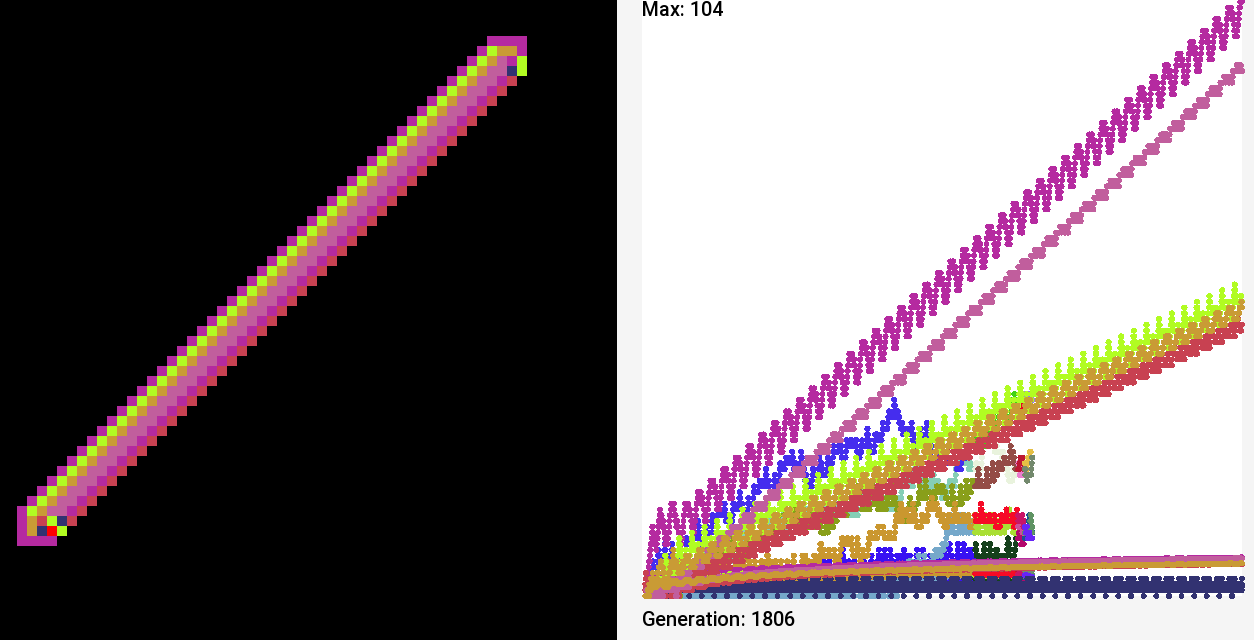
\includegraphics[width=1.2\textwidth]{img/rrrlll1.png}
	\end{minipage}%
	\vspace{0.3cm}
	
	\begin{minipage}{0.9\textwidth}
		\centering
		\small La regla RRRLLL genera una carretera que tarda el doble de tiempo en formarse en comparación con la regla LLR.
	\end{minipage}
	
	\caption{Comparación de comportamientos según diferentes reglas.}
	\label{fig:rules}
\end{figure}

\clearpage

\subsection{Interacción de múltiples hormigas en el mismo espacio}

En un espacio con $N$ estados, es posible la coexistencia de múltiples hormigas cuyas reglas tengan la misma longitud, incluso si dichas reglas no coinciden. Sin embargo, surgen dos problemas principales:  
\begin{enumerate}
	\item Si una hormiga tiene menos reglas que los estados disponibles, no tendrá un comportamiento definido al encontrarse en un estado superior al que reconoce.  
	\item Si una hormiga tiene más reglas que los estados disponibles, generará estados inaccesibles para las demás hormigas, dificultando su interacción con el entorno compartido.  
\end{enumerate}

Para abordar estas limitaciones, se proponen las siguientes soluciones:  
\begin{itemize}
	\item Si una hormiga no tiene una regla definida para un estado, avanza en línea recta mientras cambia el estado de la casilla.  
	\item Si una hormiga tiene más reglas que los estados disponibles, sus reglas se restringen al número de estados definidos en el espacio.  
\end{itemize}

Estas soluciones permiten observar nuevos comportamientos, como hormigas que avanzan en línea recta. En la Figura \ref{img:rl_3}, se ilustra el movimiento de una hormiga con la regla RL en un espacio de tres estados.

\begin{figure}[H]
	\centering
	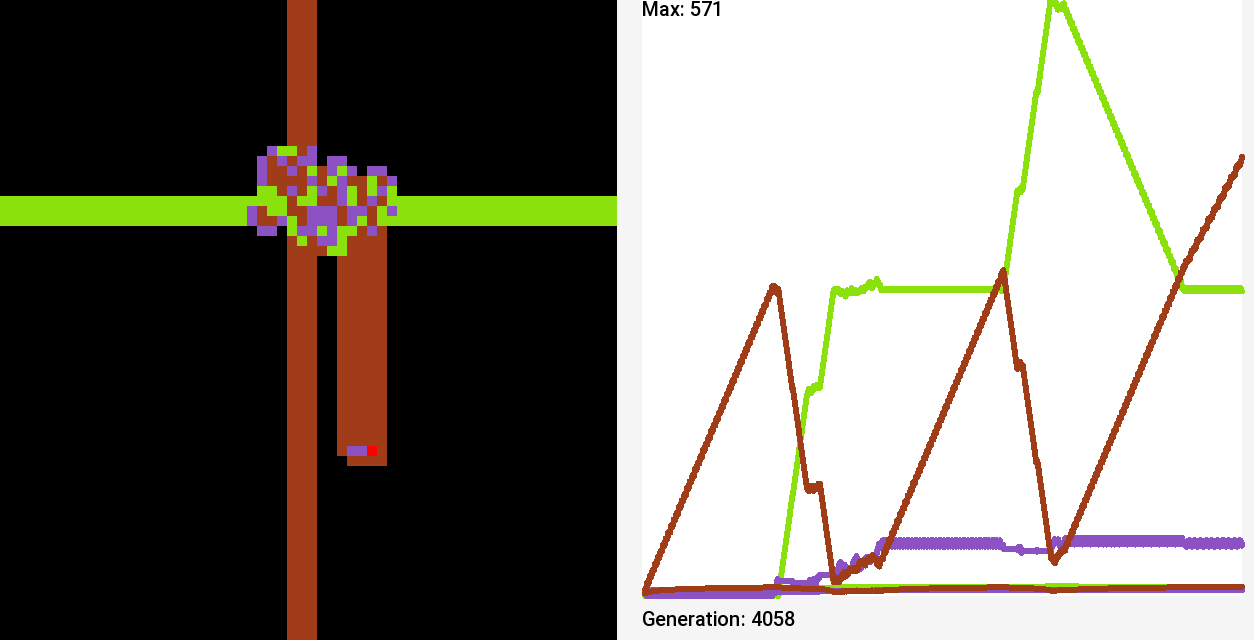
\includegraphics[width=\textwidth]{img/rl_3d.png}
	\caption{Hormiga con regla RL en un espacio con 3 estados.}
	\label{img:rl_3}
\end{figure}

\subsubsection{Misma regla}

El comportamiento pseudoaleatorio característico de la hormiga de Langton se intensifica cuando interactúan múltiples hormigas, como se observa en la Figura \ref{img:mul1}. Sin embargo, dependiendo de la configuración inicial, pueden emerger dos patrones distintivos. 

\begin{figure}[h]
	\centering
	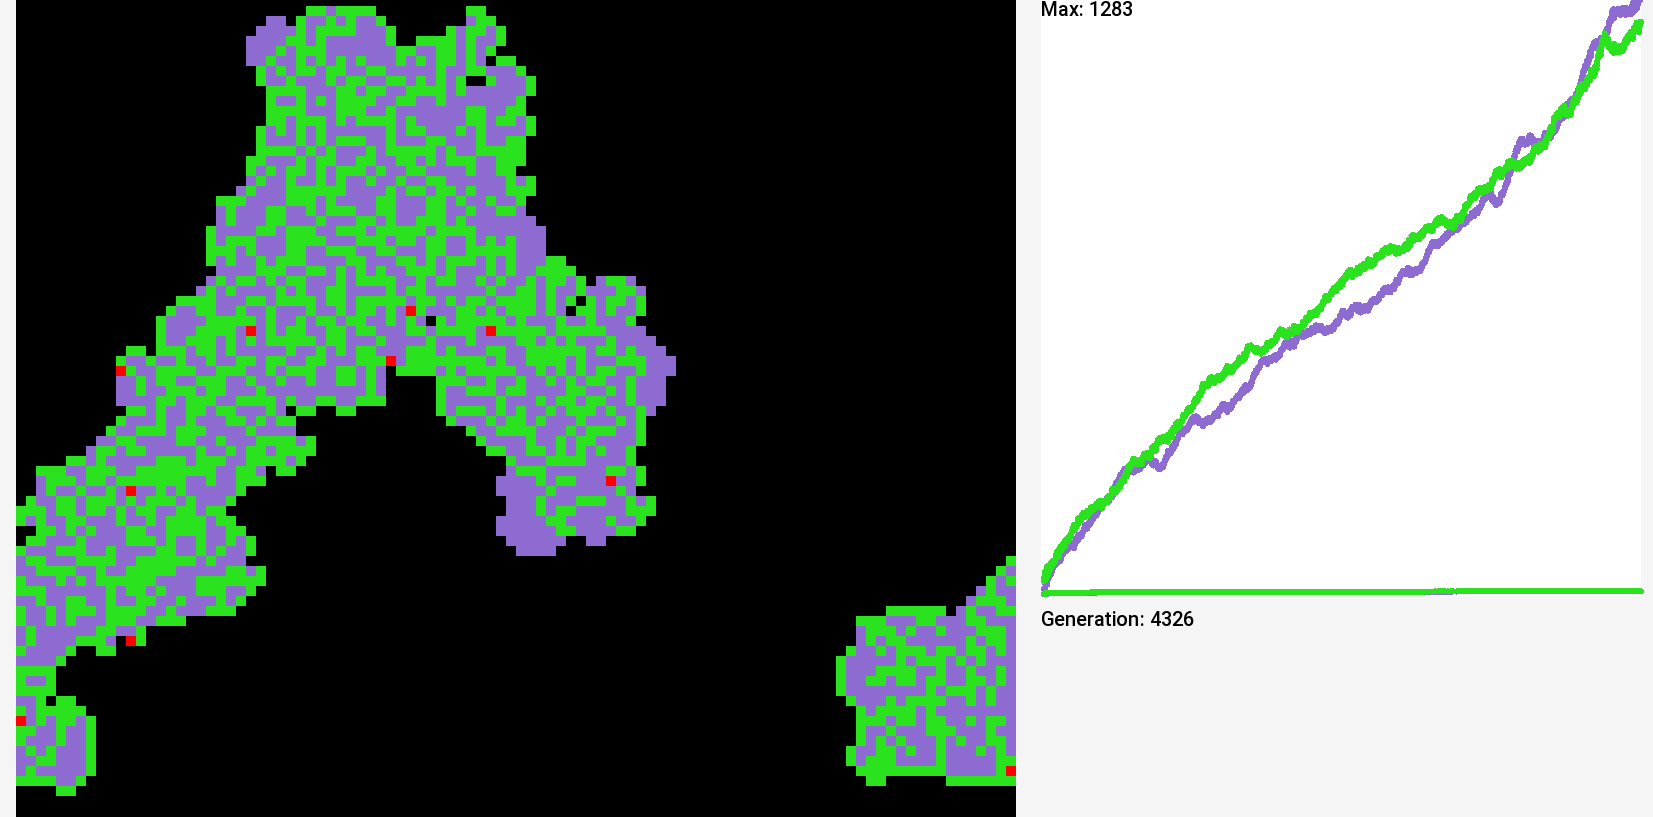
\includegraphics[width=\textwidth]{img/mul1.png}
	\caption{Interacción de múltiples hormigas con regla RL.}
	\label{img:mul1}
\end{figure}

\begin{itemize}
	\item \textbf{Construcción de carreteras}: El comportamiento caótico inicial puede derivar en la construcción de una carretera antes de alcanzar los 10,000 pasos. Un ejemplo de este fenómeno se ilustra en la Figura \ref{img:2rl}.  
	
	\begin{figure}[h]
		\centering
		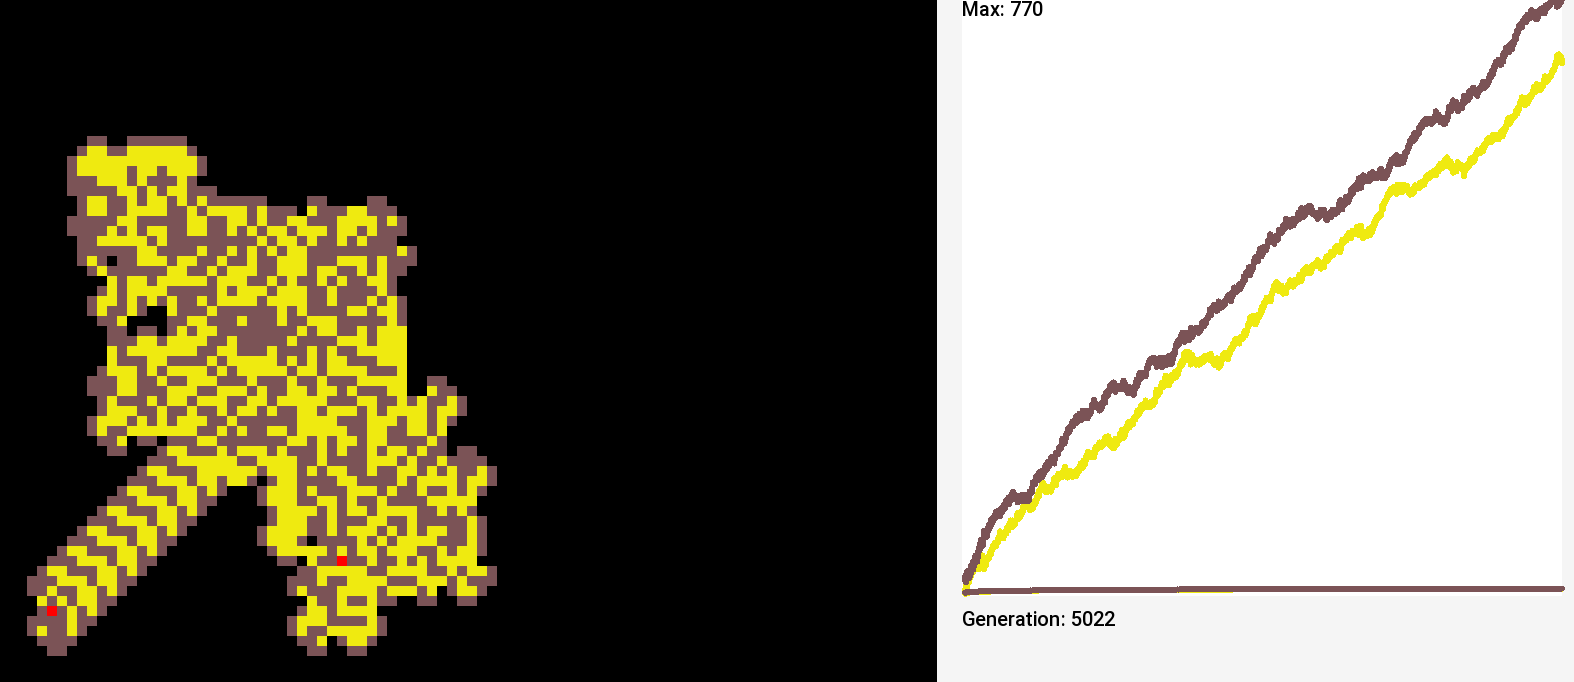
\includegraphics[width=\textwidth]{img/2rl.png}
		\caption{Construcción de una carretera por dos hormigas con regla RL.}
		\label{img:2rl}
	\end{figure}
	
	\item \textbf{Ciclos}: Colocando dos hormigas en posiciones específicas, es posible generar comportamientos periódicos, como se muestra en la Figura \ref{fig:pat}.  
	Cabe destacar que obtener un ciclo no es complicado: basta con duplicar una hormiga y posicionarla cerca, ya sea en la misma dirección o en direcciones opuestas.  
\end{itemize}

	
	La interacción de múltiples hormigas en el mismo espacio puede provocar colisiones, es decir, situaciones en las que dos hormigas intentan ocupar la misma casilla. Para resolver este problema, se selecciona al azar una hormiga que ocupará la casilla, evitando que dos hormigas compartan la misma posición. \\ \\

\begin{figure}[h!]
	\centering
	\begin{minipage}{0.45\textwidth}
	\centering
	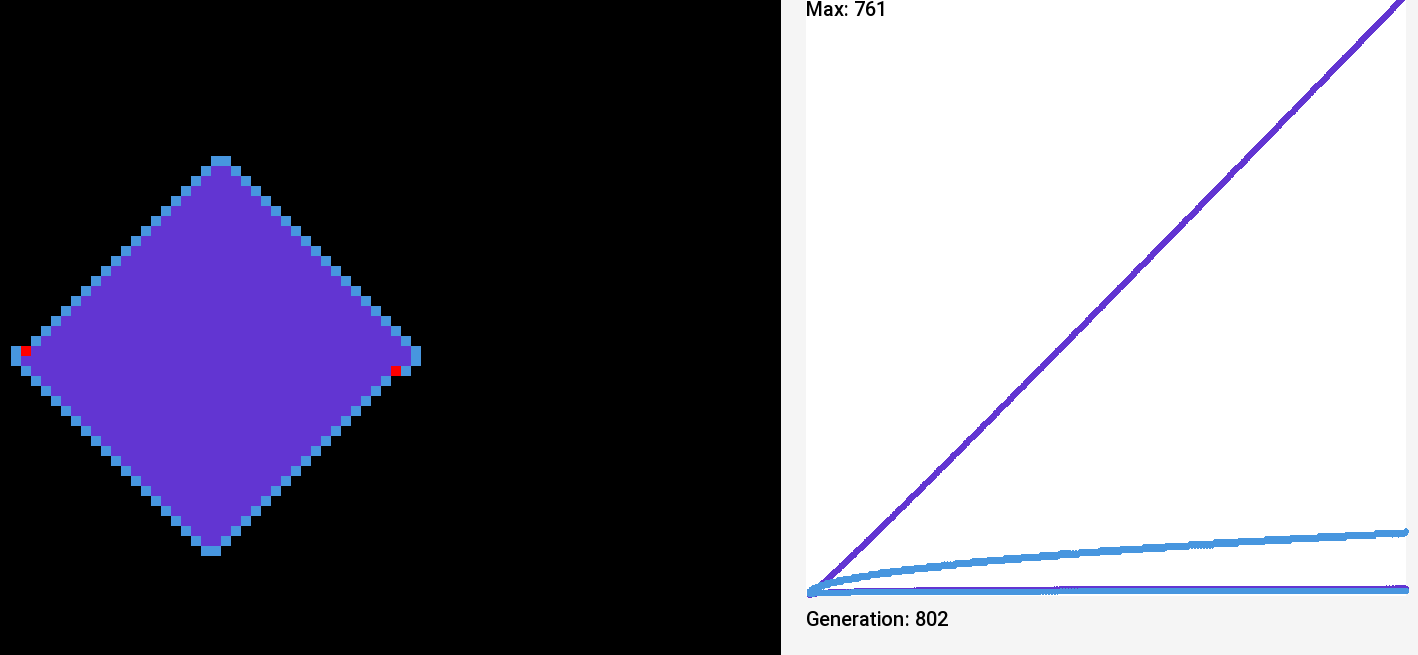
\includegraphics[width=1.4\textwidth]{img/2rl_1.png}
\end{minipage}%
\vspace{0.3cm}

\begin{minipage}{0.9\textwidth}
	\centering
	\small Dos hormigas separadas por $(1, 0)$ y orientadas en la misma dirección son capaces de modificar toda la región accesible del espacio. 
\end{minipage}
\vspace{0.5cm}
\end{figure}

\begin{figure}[h!]
	\centering
	% Primera fila

	\begin{minipage}{0.45\textwidth}
		\centering
		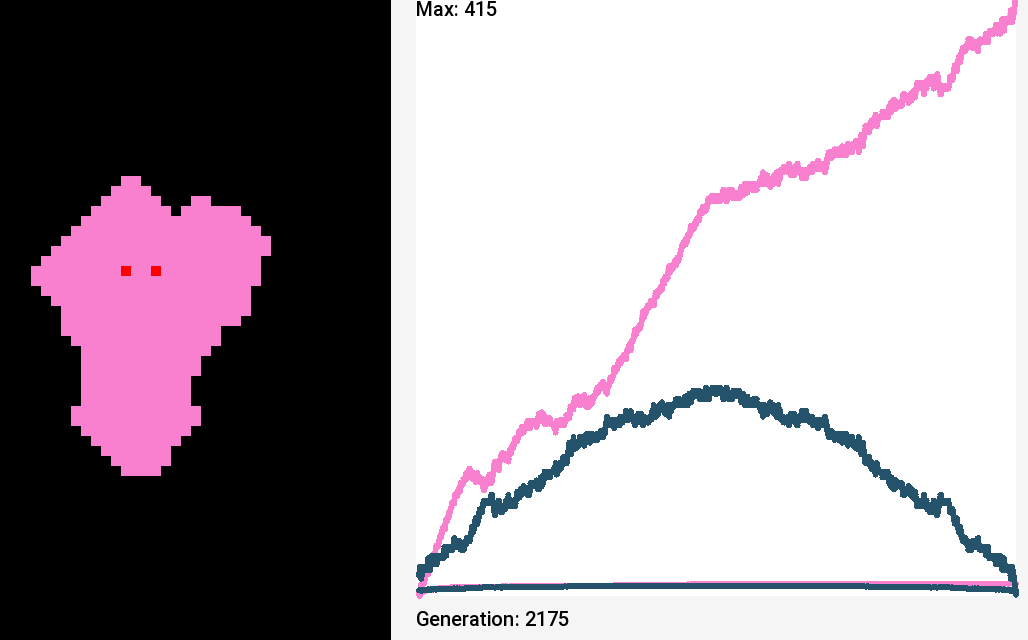
\includegraphics[width=\textwidth]{img/2_rl_1.png}
	\end{minipage}%
	\hspace{0.5cm}%
	\begin{minipage}{0.45\textwidth}
		\centering
		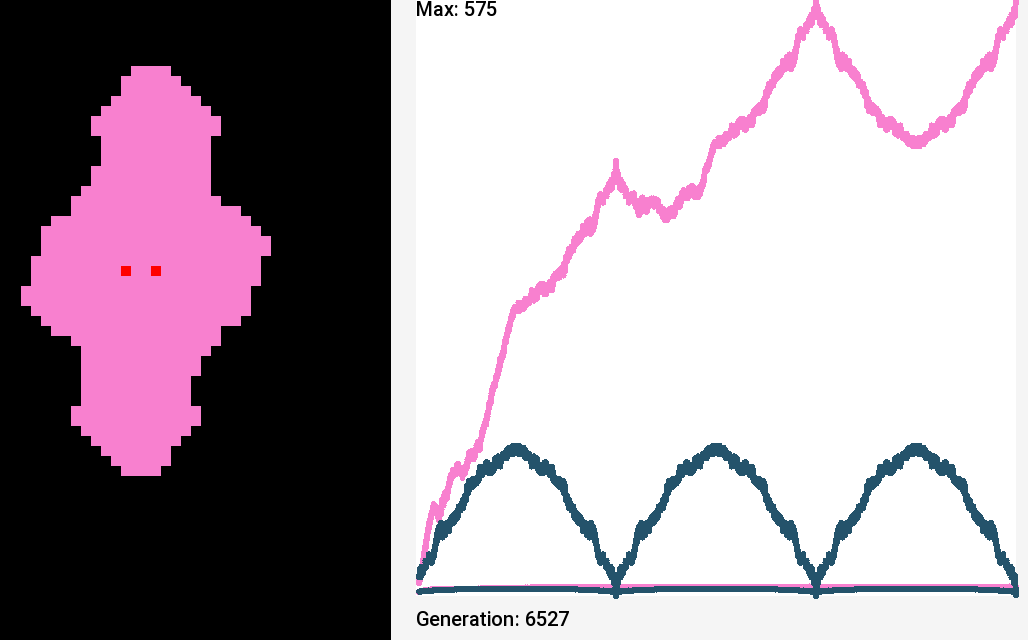
\includegraphics[width=\textwidth]{img/2_rl_2.png}
	\end{minipage}
	\vspace{0.3cm}
	
	\begin{minipage}{0.9\textwidth}
		\centering
		\small Por otro lado, si están separadas por $(+2, 0)$, generan un ciclo con un periodo de 2,175 pasos.  
	\end{minipage}
	\vspace{0.5cm}
	
	% Segunda fila
	\begin{minipage}{0.45\textwidth}
		\centering
		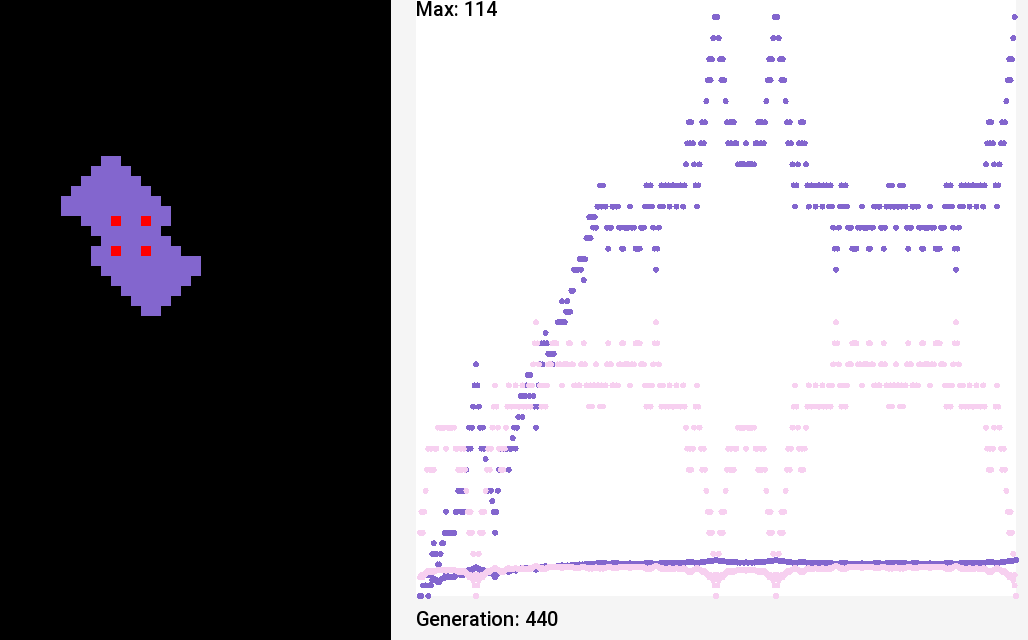
\includegraphics[width=1.4\textwidth]{img/4_rl_1.png}
	\end{minipage}
	\vspace{0.3cm}
	
	\begin{minipage}{0.9\textwidth}
		\centering
		\small Cuatro hormigas RL ubicadas en las posiciones iniciales $A_1(0, 0, U)$, $A_2(3, 0, U)$, $A_3(0, 3, D)$ y $A_4(3, 3, D)$ generan un ciclo con un periodo de 220 generaciones.  
	\end{minipage}
	
	\caption{Patrones periódicos generados por múltiples hormigas con regla RL.}
	\label{fig:pat}
\end{figure}

\clearpage
\subsubsection{Multiples reglas}
Como ya se menciono, multiples hormigas pueden coexistir en el mismo espacio. En la figura \ref{fig:rules_mul} se muestran varias de estas configuraciones:
\begin{figure}[h!]
	\centering
	% Primera fila
	
	\begin{minipage}{0.6\textwidth}
		\centering
		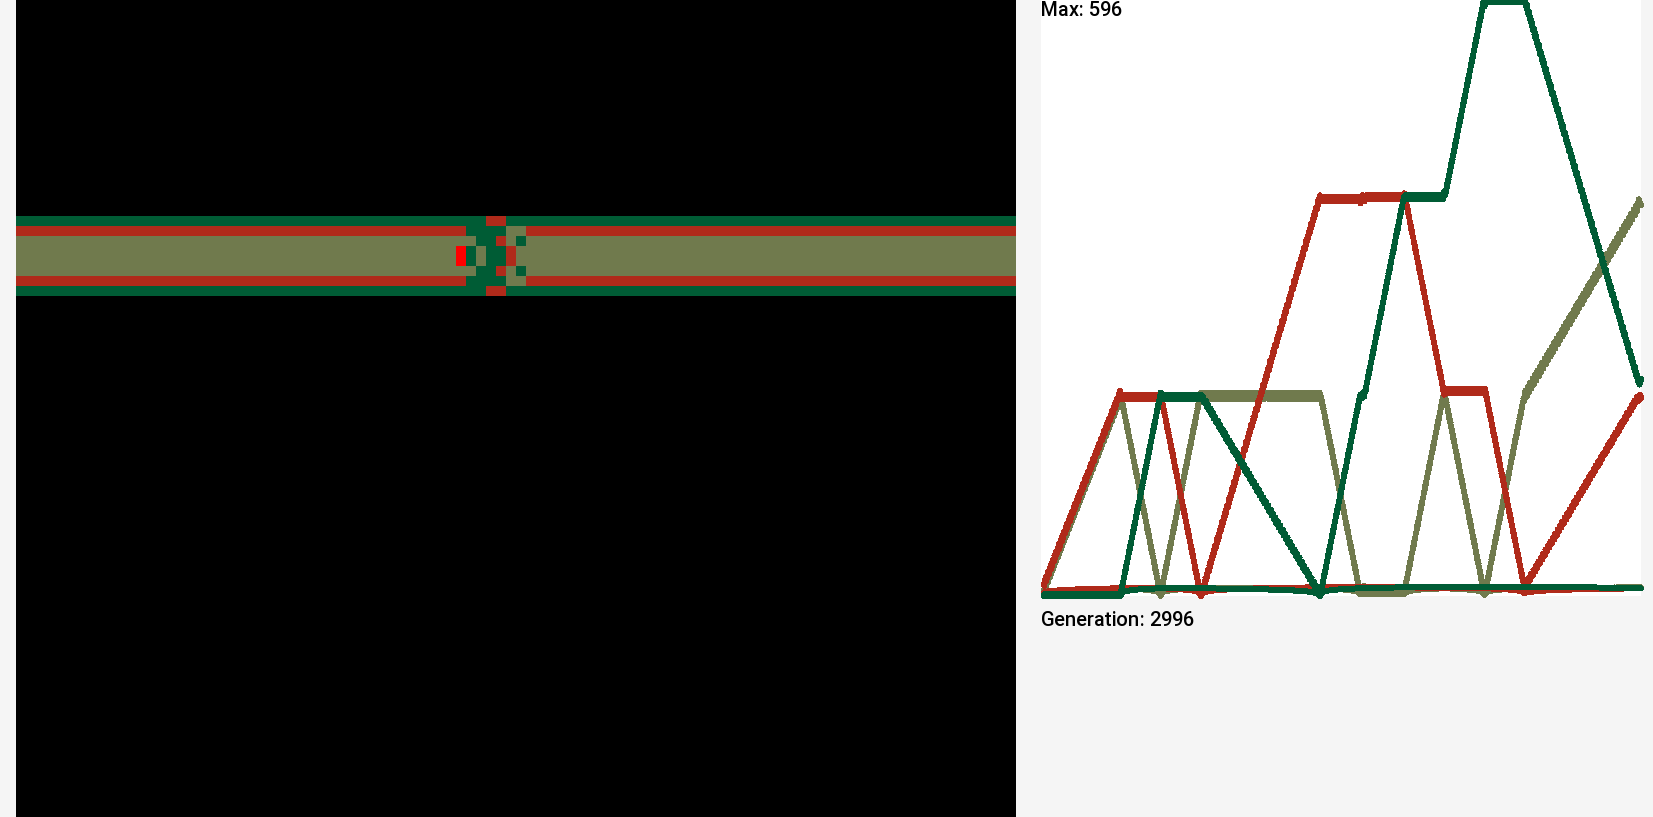
\includegraphics[width=1.3\textwidth]{img/mul_1.png}
	\end{minipage}%
	\vspace{0.3cm}
	
	% Segunda fila
	\begin{minipage}{0.6\textwidth}
		\centering
		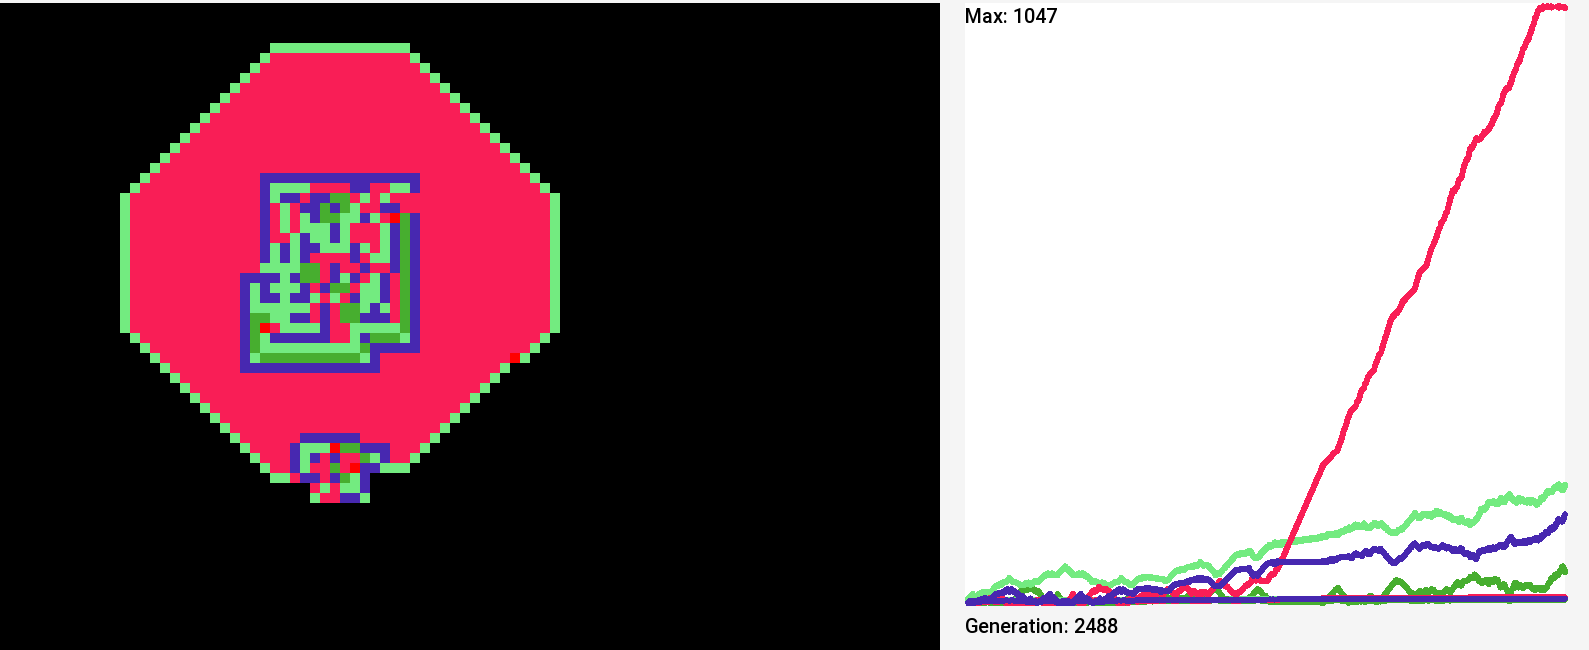
\includegraphics[width=1.3\textwidth]{img/mul_2.png}
	\end{minipage}
	\vspace{0.3cm}
	
	% Segunda fila
	\begin{minipage}{0.6\textwidth}
		\centering
		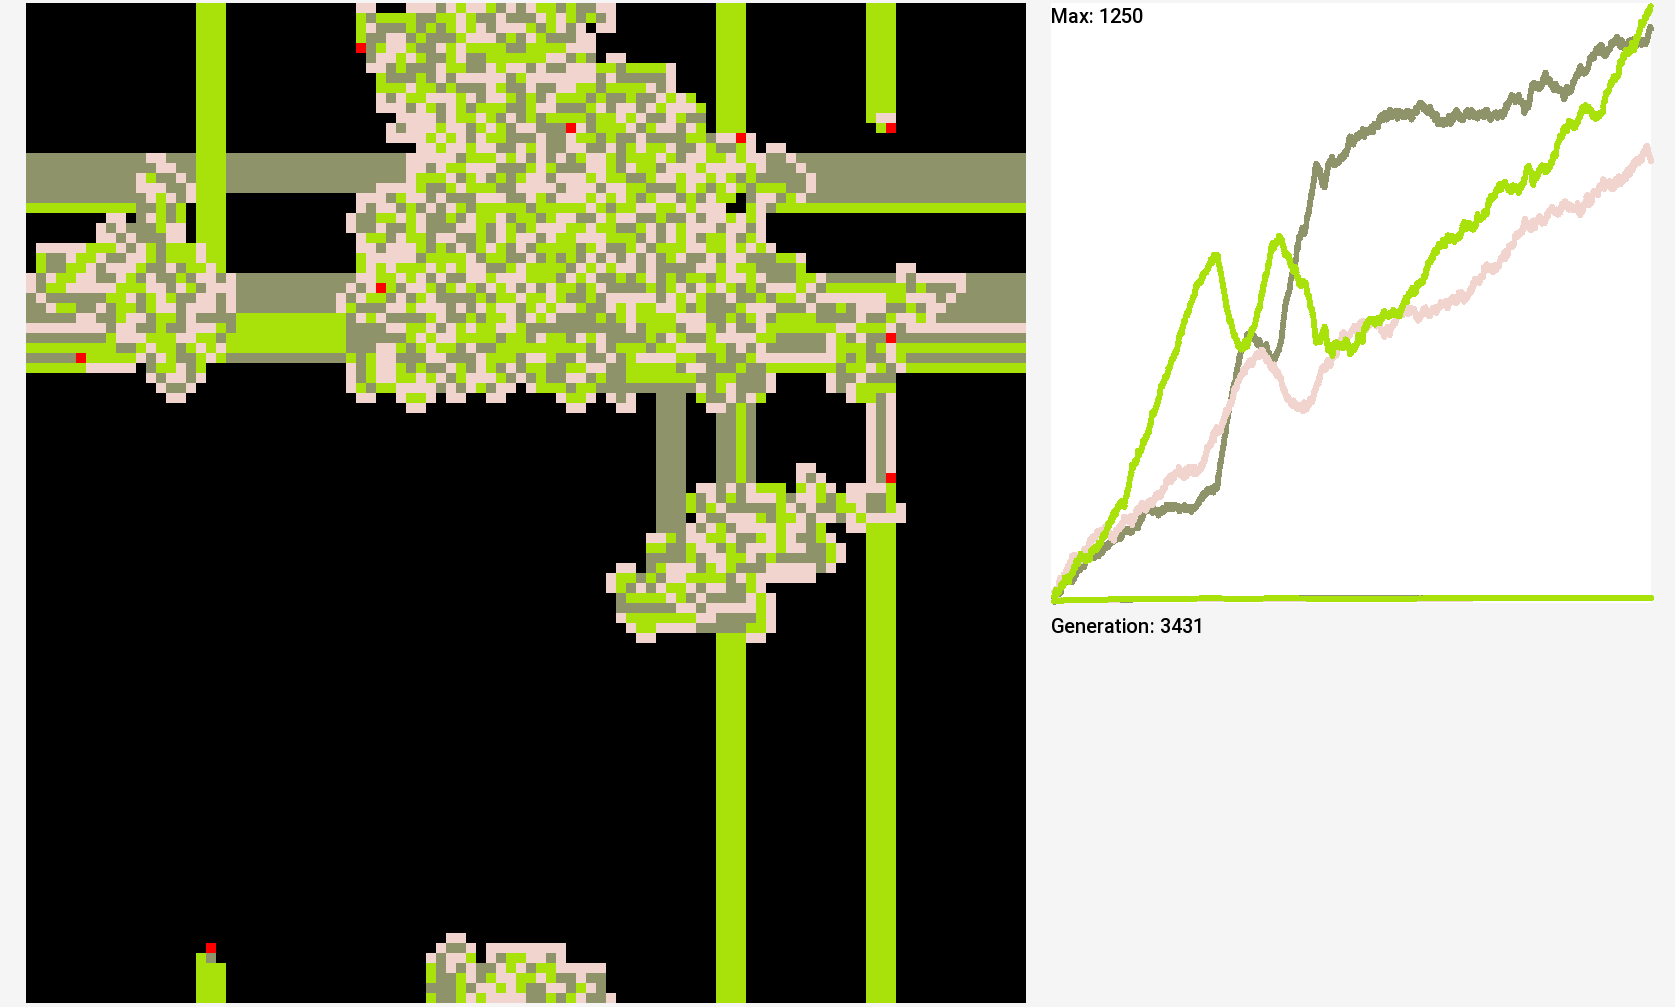
\includegraphics[width=1.3\textwidth]{img/mul_3.png}
	\end{minipage}
	\vspace{0.3cm}

	\caption{Patrones periódicos generados por múltiples hormigas con regla RL.}
	\label{fig:rules_mul}
\end{figure}

\clearpage
\section{Hormigueros}


	\clearpage
	\addcontentsline{toc}{section}{Referencias}
	\begin{thebibliography}{99}
		\bibitem{}
		
	\end{thebibliography}
	
\end{document}
